\documentclass[12pt]{article}
\usepackage[utf8]{inputenc}
\usepackage[russian]{babel}
\usepackage{graphicx}
\graphicspath{ {./images/} }

\begin{document}

\textit{\textbf{Задание 11.}}

\textit{Постройте релейно-контактную схему с заданной функцией
проводимости:}

$$(x \rightarrow (y \rightarrow z)) \rightarrow (y \rightarrow x')$$

\underline{Решение:}

Выразим сначала данную функцию через функции $', \cdot , \lor$, причем так,
чтобы знак $'$ стоял бы лишь на переменных и не стоял на скобках:

$$(x \rightarrow (y \rightarrow z)) \rightarrow (y \rightarrow x') = (x' \lor (y' \lor z))' \lor (y' \lor x') = $$

$$ = xyz' \lor y' \lor x'.$$

Соответствующая схема имеет вид

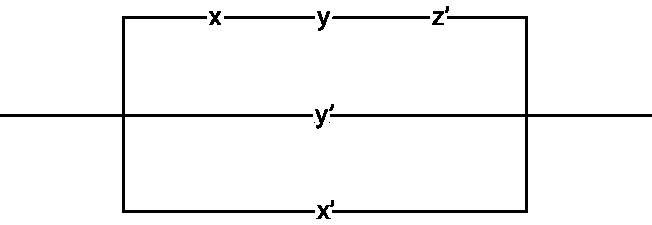
\includegraphics{11_1.pdf}

Обратим внимание, что данную схему можно еще упросить

$$ xyz' \lor y' \lor x' = x' \lor y' \lor z'.$$

Тогда схема будет иметь вид:

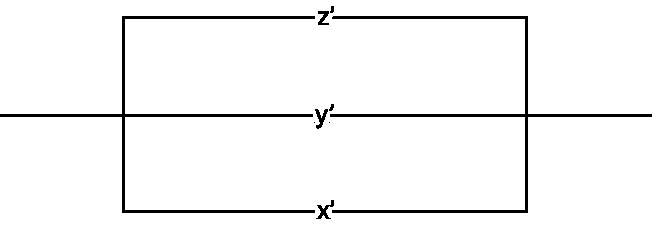
\includegraphics{11_2.pdf}

\pagebreak

\textit{\textbf{Задание 12}}

\textit{Упростите релейно-контактную схему:}

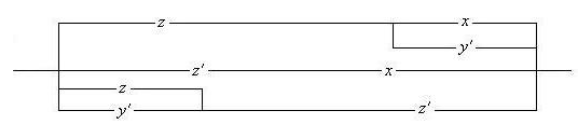
\includegraphics[scale=0.5]{12_1}

$$f=z(x \lor y') \lor z'x \lor (z \lor y')z'$$

$$f=z(x \lor y') \lor z'x \lor (z \lor y')z' = xz \lor y'z \lor xz' \lor y'z' =$$
$$ = x \lor y' $$

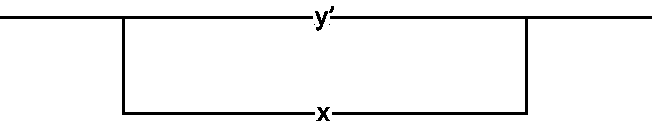
\includegraphics{12_2}

\end{document}
